\chapter{CMS Particle and Event Reconstruction}
After an event is chosen to be stored by the trigger system, the output from all of the sub-detectors is saved and recorded to disk as "RAW" data.  These data contain information about the response of each sub-detector, such as tracker hits and energy deposition in the calorimeters.  As was mentioned in Chapter 4, shown in Table \ref{table:subdetsignals} and Figure \ref{fig:cmsslicewhitecolourfrench291016}, the CMS was designed such that each type of particle resulting from the $pp$ collisions at the IP would leave a distinct signature in the sub-detectors.  This allows for the information to be reconstructed into lists of physics object candidates such as photons, electrons, muons, etc and quantities such as missing transverse momentum.  The particle flow (PF) algorithm performs this reconstruction by first building tracks and calorimeter clusters.  These two elements are the inputs to the reconstruction of the aforementioned physics object candidates using a "link" algorithm.

\section{Tracks}
A combinatorial track finder algorithm based on the Kalman filtering technique uses the hits in the silicon tracker to reconstruct tracks of charged particles \cite{Kalmantracking:1987fm}.  Each iteration of the algorithm is comprised of three steps:
\begin{itemize}
	\item Seed generation:  Find a seed consisting of two to three hits that is compatible with a track from a charged particle.
	\item Track finding: Use pattern recognition to identify any hits that are compatible with the trajectory implied by the seed generated in the first step.
	\item Track fitting: Determine the properties of the track, such as origin, trajectory, and transverse momentum by performing a global $\chi^2$ fit.
\end{itemize}

The first iteration uses stringent requirements on the seeds and the $\chi^2$ of the track fit to pick out isolated jets which have very high purity.  The hits associated with these high purity tracks are then removed to reduce the combinatorial complexity for subsequent iterations.  This allows successive iterations to identify less obvious tracks by progressively loosening criteria while the removal of previously associated hits mitigates the likelihood of fake tracks being built.  


\section{Calorimeter clusters}
Calorimeter clusters are constructed using energy deposition information from the calorimeters.  Clusters are formed by first identifying the seed cell (ECAL crystal or HCAL scintillating tile) that corresponds to the local maxima of an energy deposit that is above a given threshold.  Neighboring cells are then aggregated to grow topological clusters if their signals are above twice the standard deviation of the level of electronic noise.  

\section{Object identification}
At this point the tracks and calorimeter clusters are linked to form a PF block.  This linkage is done with an algorithm that quantifies the likelihood that a given track and cluster were results of the same particle.  As PF blocks are identified as object candidates they are removed from the collection prior to each subsequent iteration until all tracks and clusters have been assigned to a PF object candidate.  The following sections will outline how each of these PF objects is identified.
\subsection{Muons}
Muons are the easiest particle to identify, so they are the first objects reconstructed in the CMS.  PF Muons are classified in three categories depending on how their tracks are reconstructed:
\begin{itemize}
	\item Tracker muons:  Tracks reconstructed from the inner tracker having $p_T>0.5$ GeV and $|\vec{p}|>2.5$ GeV that, when propagated to the muon system, match at least one hit in the muon chambers.
	\item Stand-alone muons:  Tracks reconstructed only using hits in the muon system.
	\item Global muons:  Stand-alone muons that coincide with a track from the inner tracker.
\end{itemize}
After a muon is reconstructed it is given an identification or ID based on observables such as the $\chi^2$ of the track fit, how many hits were recorded per track, or how well the tracker and stand-alone tracks matched.  These IDs represent different working points (loose, medium, and tight) which correspond to increasing purity but decreasing efficiency as you move from loose toward tight.  
\subsection{Electrons}
The next objects reconstructed in the CMS are electrons.  Bremsstrahlung in the tracker layers causes substantial energy loss and changes in momentum which requires the use of a dedicated tracking algorithm.  In place of the Kalman filtering technique, a Gausian-sum filter (GSF) algorithm is used.  This algorithm uses a weighted sum of Gaussian PDFs which does a better job of modeling the Bremsstrahlung effects than the Kalman filtering technique which uses a single Gaussian PDF.  

PF ECAL clusters are regrouped by identifying a seed cluster then associating and adding clusters from Bremsstrahlung photons to form superclusters.  The schematic in Figure \ref{fig:electrontracking} shows how the Bremsstrahlung photons are emitted in directions tangent to the trajectory of the electron.  Electrons bending in the magnetic field causes spreading of PF ECAL clusters to typically occur along the $\phi$-direction.  Two approaches are used to associate the superclusters to GSF tracks.  One is the ECAL-driven method, which uses superclusters with $p_T > 4$ GeV as seeds for the GSF track finding algorithm.  This works well for high-$p_T$ isolated electrons because the bend radius is less severe which decreases the spread of the PF ECAL clusters. This results in more of the Bremsstrahlung radiation being recovered and correctly assoiated with an electron candidate.  The second approach is the tracker-driven method which uses tracks with $p_T > 2$ GeV as seeds that are propagated out to the surface of the ECAL and used for clustering.  This method works best with soft electrons like those in jets because it relies on the high granularity of the tracker to disentangle overlapping energy deposits in the ECAL. \cite{Electrontracking:2715343}

\begin{figure}[h]
	\centering
	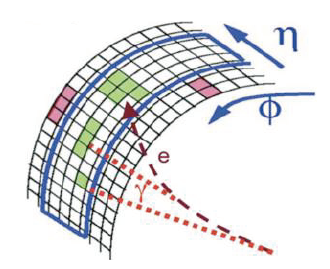
\includegraphics[width=0.4\linewidth]{Figures/electrontracking}
	\caption{The Bremsstrahlung photons continue along a straight trajectory while the electron path is bent by the magnetic field.  This results in energy deposited in the calorimeter for such electrons to be spread out along the $\phi$-direction.}
	\label{fig:electrontracking}
\end{figure}

As a final step, a boosted decision tree (BDT) is used to discriminate between real and fake electrons.  The BDT is given variables associated with track-cluster matching, shower shape, and tracking.  The output score of the BDT is used to classify electrons into loose, medium, and tight working points which exhibit to the same purity and efficiency trends as the muon working points.

\subsection{Photons} 
Unlike electrons, photons typically deposit most of their energy in the ECAL without interacting with the tracker therefore their reconstruction is seeded from ECAL superclusters that do not have any GSF tracks associated with them.  When photons interact with the tracker material they convert into electron-positron pairs which follow bent trajectories due to the magnetic field prior to entering the ECAL.  This causes a spread of the energy deposition along the $\phi$-direction.  The goal of the clustering algorithm for photon reconstruction is to include all of the energy deposits of electrons resulting from photon conversions.  As with the calorimeter clustering algorithm, the photon clustering starts by identifying a local energy maxima as a seed crystal. In the EB a cluster is made up of several parallel strips of crystals $5\times1$ in $\eta \times \phi$.  The first strip has the seed crystal at its center.  Neighboring strips in the $\phi$-direction are added if they have energy above a threshold of 10 GeV but less than that of the subsequent strip with a maximum of 17 strips in a cluster.  In the EE, the seed cluster is $5\times5$ with adjacent $5\times5$ clusters being added if they meet the minimum energy requirement.

Converted and unconverted photons can be differentiated by looking at how the energy is distributed in a supercluster.  The variable $R_9$ is used for this purpose.  It is defined as the ratio of the energy in a $3\times3$ crystal array to the energy in the entire supercluster.  As the energy deposits resulting from converted electrons is more spread out they result in a lower $R_9$ value than unconverted photons.  A photon is candidate is considered to be unconverted when $R_9>0.93$.  

An important point regarding the clustering algorithm is that it does not differentiate between showers resulting from photons and those resulting from electrons.  This allows for electron from $Z\rightarrow ee$ events to be used as high purity samples to study analysis inputs and for defining control regions using electron in place of photons.


\subsection{Jets}
When quarks or gluons are produced they hadronize to make cone-shaped, collimated collections of particles called jets.  The jet clustering algorithm aims to combine these particles in order to accurately measure the kinematics of the initial gluon or quark.  The algorithm uses the two distance parameters
\begin{eqnarray}
	d_{ij} &=& min(k_{T_i}^{2p},k_{T_j}^{2p})\frac{\Delta R_{ij}^2}{R^2} \\
	d_{iB} &=& k_{T_i}^{2p}
\end{eqnarray}
where $d_{ij}$ is the distance between objects $i$ and $j$ and $d_{iB}$ is the distance between object $i$ and the beam $B$.  The transverse momentum of the object is $k_T$.  The parameter $p$ is set either -1, 0, or +1 to specify whether the anti-$k_T$, inclusive Cambridge/Aachen, or inclusive $k_T$ algorithm is used, respectively.  The value of $\Delta R_{ij}^2$ is defined as $(\eta_i-\eta_j)^2+(\phi_i-\phi_j)^2$ and $R$ is the distance parameter that defines the radius of the jet.

his analysis uses jets reconstructed from PF candidates using the anti-$k_T$ algorithm with $R= 0.4$, also known as AK4PFJets or just PFJets. The algorithm goes through the following steps:
\begin{enumerate}
	\item The smallest values of $d_{ij}$ and $d_{iB}$ are computed for all objects in the event.
	\item Objects $i$ and $j$ are merged into a single object if $d_{ij}<d_{iB}$.  
	\item Object $i$ is labeled as a jet and removed from the list if $d_{iB}<d_{ij}$. 
\end{enumerate}

Note for next time:  
Now talk about infrared and collinear safe.  Use Allie's thesis for guide.
Look at "recent thesis" for ECAL noise on 2017 data.
Should also do JEC and JER in here. 


\section{Missing transverse momentum}

